
\usepackage{fancyhdr}
\usepackage{lastpage}
\usepackage[utf8]{inputenc}

% Minted for syntax highliting
\usepackage{minted}
\usemintedstyle{tango}

% 
\usepackage[T1]{fontenc}
\usepackage{lmodern}

\usepackage{calc}
\usepackage{bytefield}

\usepackage{listings}
\usepackage{amsmath}

\usepackage{tikz}
\usetikzlibrary{automata,arrows,topaths,calc,positioning}
 
\usepackage{syntax}
\grammarindent=2cm


% Headers/footers styling
\pagestyle{fancy}
\fancyhf{}
\renewcommand{\headrulewidth}{0pt}

% Footer
\lfoot{ID1019}
\cfoot{KTH}
\rfoot{\thepage \hspace{1pt} / \pageref{LastPage}}

%\newcommand{\defaultpagestyle}{\thispagestyle{plain}}
\newcommand{\defaultpagestyle}{\thispagestyle{fancy}}



\title[ID1019 A transport layer]{A transport layer}


\author{Johan Montelius}
\institute{KTH}
\date{\semester}

\begin{document}

\begin{frame}
\titlepage
\end{frame}

\begin{frame}{Communication service}

  Assume we have a communication channel that allow us to send {\em
    frames} between two connected nodes. The channel is not reliable
  so messages can be lost or delivered out of order. \pause ..... 

\vspace{20pt}
\pause We want to build a communication service that is ..... \pause better.

\pause
\vspace{20pt}

Our task is to build a communication service that provides: \pause

\begin{itemize}

\item reliable delivery: despite frames being lost \pause

\item ordered delivery: FIFO - first-in-first-out \pause

\item identity: an addressing scheme \pause

\item flow control: prevented from overflowing a receiver  

\end{itemize}


\end{frame}

\begin{frame}{layered architecture}

Build a solution using a layered architecture. 

\vspace{20pt} \pause

Each layers provides an {\em abstraction} that the layer above can make use of.

\end{frame}

\begin{frame}{layers}

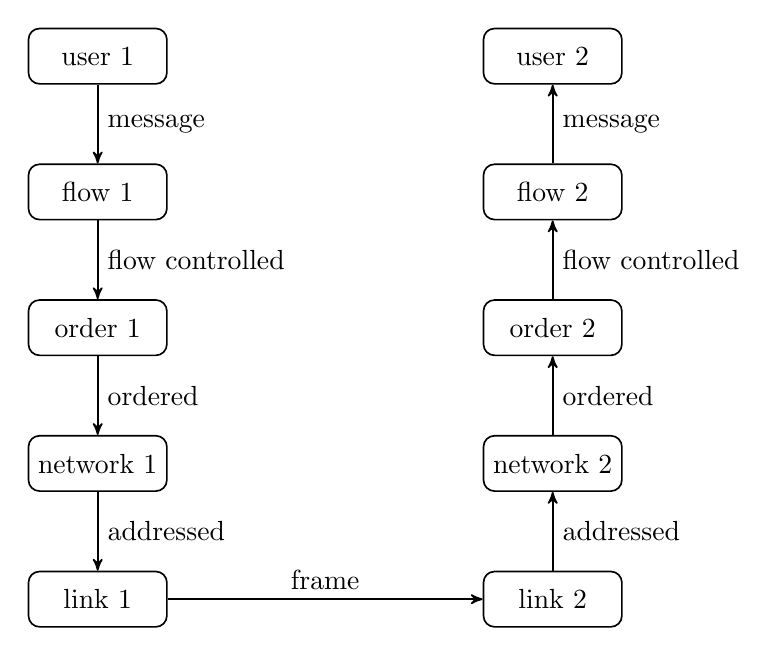
\begin{tikzpicture}[>=stealth', semithick, auto]

    \tikzstyle{fbp} = [rectangle, rounded corners, minimum width=50pt, minimum height=20pt, text centered, draw=black]        


    \node (user1)  [fbp]                                 {user 1};
    \node (user2)  [fbp, right=4cm of user1]             {user 2};            
    
    \node (flow1)  [fbp, below=1cm of user1]             {flow 1};
    \node (flow2)  [fbp, below=1cm of user2]             {flow 2};        

    \node (order1) [fbp, below=1cm of flow1]             {order 1};
    \node (order2) [fbp, below=1cm of flow2]             {order 2};        

    \node (netw1)  [fbp, below=1cm of order1]            {network 1};
    \node (netw2)  [fbp, below=1cm of order2]            {network 2};

    \node (link1)  [fbp, below=1cm of netw1]             {link 1};
    \node (link2)  [fbp, below=1cm of netw2]             {link 2};    

    \path[->]  (user1)    edge        node         {message}       (flow1);
    \path[<-]  (user2)    edge        node         {message}       (flow2);
    
    \path[->]  (flow1)    edge        node         {flow controlled}       (order1);
    \path[<-]  (flow2)    edge        node         {flow controlled}       (order2);
    
    \path[->]  (order1)   edge        node         {ordered}       (netw1);
    \path[<-]  (order2)   edge        node         {ordered}       (netw2);

    \path[->]  (netw1)   edge        node          {addressed}       (link1);
    \path[<-]  (netw2)   edge        node          {addressed}       (link2);

    \path[->]  (link1)   edge        node          {frame}       (link2);

\end{tikzpicture}


\end{frame}


\begin{frame}{the link layer}


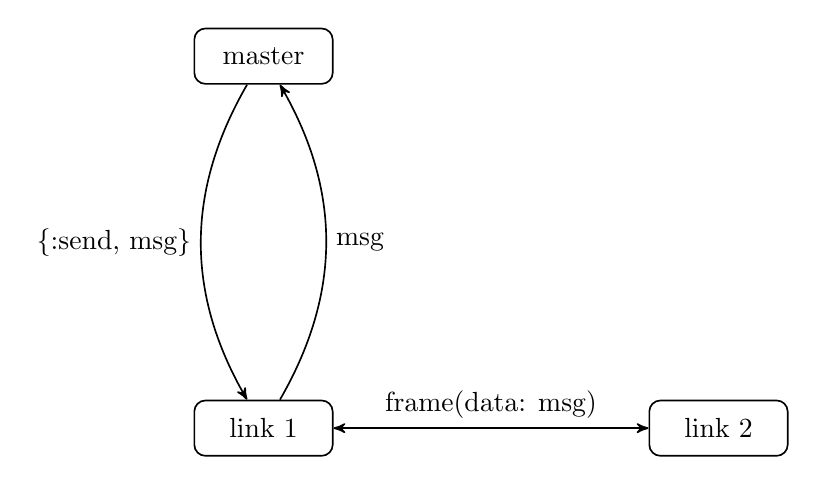
\begin{tikzpicture}[>=stealth', semithick, auto]

    \tikzstyle{fbp} = [rectangle, rounded corners, minimum width=50pt, minimum height=20pt, text centered, draw=black]        


    \node (master)  [fbp]                                 {master};

    \node (link1)  [fbp, below=4cm of master]            {link 1};

    \node (link2)  [fbp, right=4cm of link1]            {link 2};    

    \path[->, bend right]  (master)   edge        node[anchor=east]          {\{:send, msg\}}       (link1);
    \path[->, bend right]  (link1)   edge        node[anchor=west]          {msg}       (master);
    \path[<->]  (link1)   edge        node[above]          {frame(data: msg)}       (link2);    
\end{tikzpicture}

\end{frame}

\begin{frame}{the link process - a state diagram}
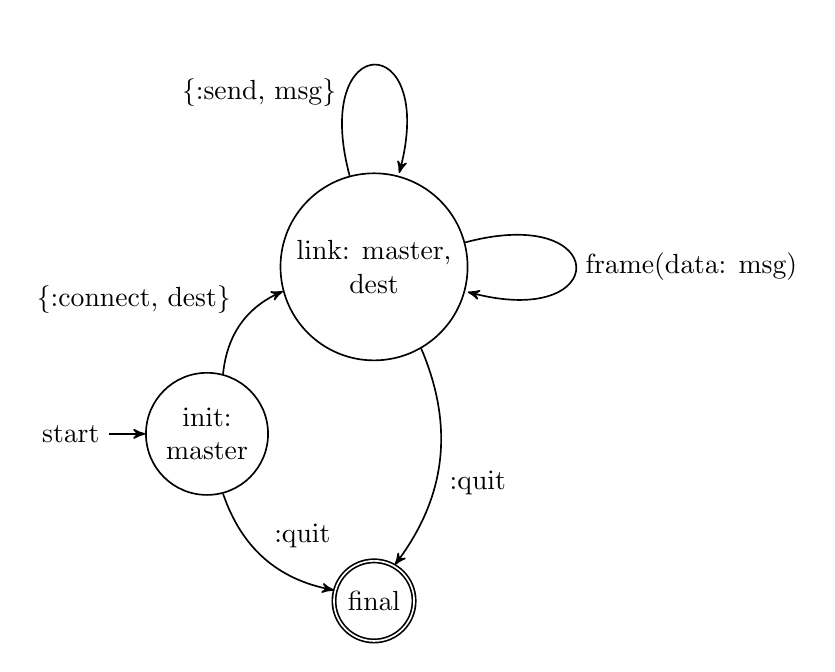
\begin{tikzpicture}[>=stealth', node distance=3cm, semithick, auto]

  \node[initial, state]            (init)    [align=center]        {init: \\master};
    \node[state]                     (link)    [align=center, above right of=init]     {link: master,\\dest};
    \node[accepting, state]          (final)   [below right of=init]     {final};


    \path[->]   (init)   edge       [bend left]     node      {\{:connect, dest\}}       (link)
                         edge       [bend right]    node      {:quit}          (final) 
                (link)   edge       [loop above]    node[near start, anchor=east]   {\{:send, msg\}}          (link)
                         edge       [loop right]    node      {frame(data: msg)}           (link)
                         edge       [bend left]     node      {:quit}          (final);
\end{tikzpicture}

\end{frame}


\begin{frame}[fragile]{the link process}

\begin{verbatim}
  require Record

  Record.defrecord(:frame, data: nil)

  def start(master) do
    {:ok, spawn(fn() -> init(master) end)}
  end

  defp init(master) do
    receive do
      {:connect, dest} ->
        link(master, dest)
      :quit ->
        :ok
    end
  end
\end{verbatim}
\end{frame}

\begin{frame}[fragile]{the link process}
\begin{verbatim}
  def link(master, dest) do
    receive  do
      {:send, msg} ->
        send(dest, frame(data: msg))
        link(master, dest)

      frame(data: msg) ->
        send(master, msg)
        link(master, dest)

      :quit ->
        :ok
    end
  end
\end{verbatim}
  
\end{frame}


\begin{frame}[fragile]{a first try}

\begin{verbatim}
def test() do 
  sender = spawn(fn() -> sender() end)
  receiver = spawn(fn() -> receiver() end)
  link1 =   Link.start(sender)
  link2 =   Link.start(receiver)
  send(link1, {:connect, link2})
  send(link2, {:connect, link1})
  send(sender, {:connect, link1})
  send(reciever, {:connect, link2})
  :ok
end
\end{verbatim}
  
\end{frame}

\begin{frame}{a hub}

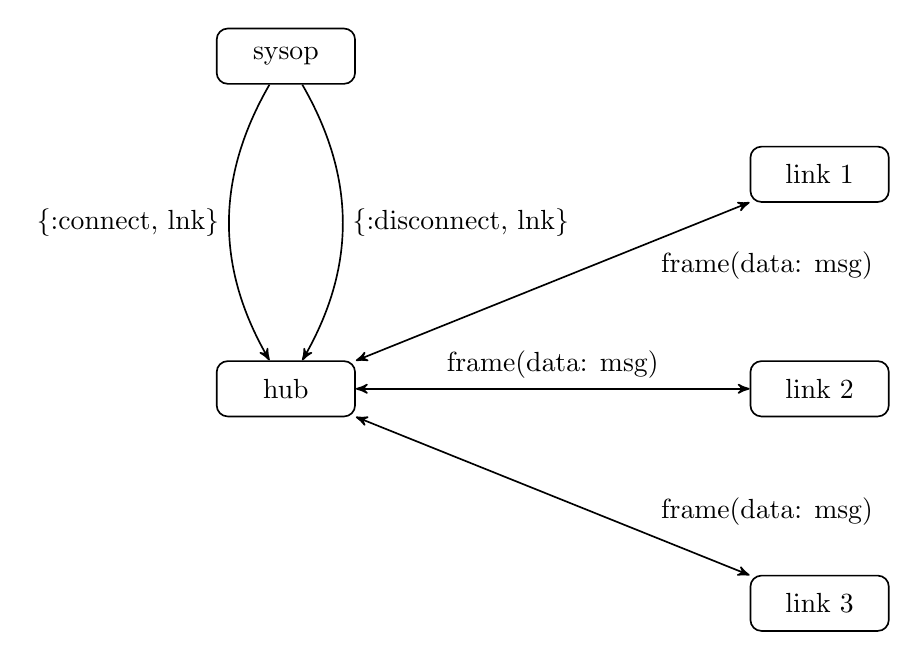
\begin{tikzpicture}[>=stealth', semithick, auto]

    \tikzstyle{fbp} = [rectangle, rounded corners, minimum width=50pt, minimum height=20pt, text centered, draw=black]        


    \node (master)  [fbp]                        {sysop};

    \node (hub)  [fbp, below=3.5cm of master]    {hub};

    \node (link2)  [fbp, right=5cm of hub]            {link 2};    
    \node (link1)  [fbp, above=2cm of link2]          {link 1};    
    \node (link3)  [fbp, below=2cm of link2]          {link 3};
    
    \path[->, bend right]  (master)   edge  node[anchor=east]  {\{:connect, lnk\}}    (hub);
    \path[->, bend left]  (master)   edge   node[anchor=west]  {\{:disconnect, lnk\}} (hub);
    \path[<->]  (hub)   edge        node[near end, above, anchor=north west]  {frame(data: msg)}       (link1);    
    \path[<->]  (hub)   edge        node[above]          {frame(data: msg)}       (link2);
    \path[<->]  (hub)   edge        node[near end, above, anchor=south west]  {frame(data: msg)}       (link3);        
\end{tikzpicture}

\end{frame}

\begin{frame}{the hub - a state diagram}

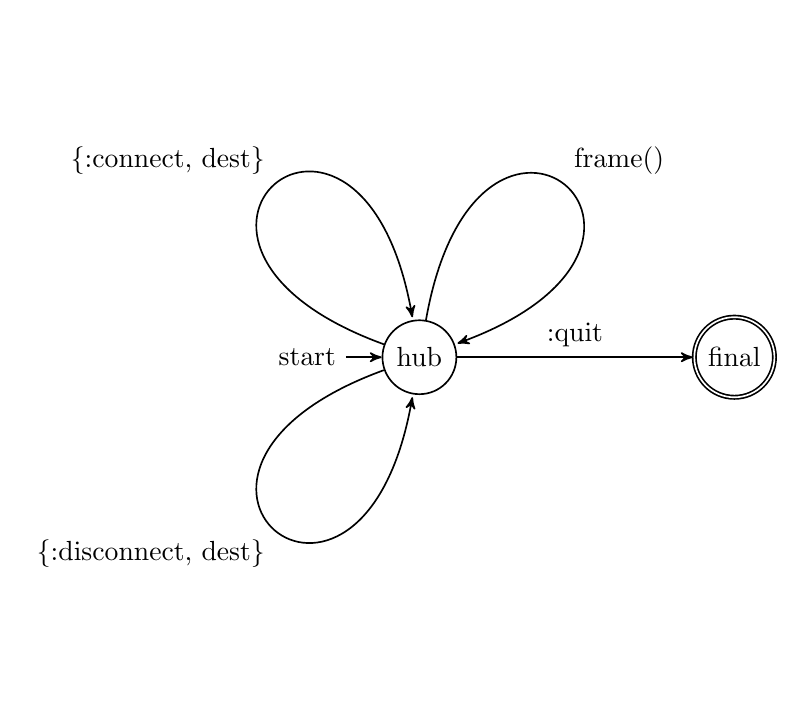
\begin{tikzpicture}[>=stealth', node distance=4cm, semithick, auto]

    \node[initial, state]            (hub)                        {hub};
    \node[accepting, state]          (final)   [right of=hub]     {final};


    
    \path[->]   (hub)   edge       [loop above, every loop/.append style={looseness=20,in=100, out=160 }]    node[anchor=south east]      {\{:connect, dest\}}       (hub)
                        edge       [loop below, every loop/.append style={looseness=20,in=260, out=200 }]    node[anchor=north east]      {\{:disconnect, dest\}}    (hub)
                        edge       [loop above, every loop/.append style={looseness=20,in=20,  out=80 }]     node[anchor=south west]      {frame()}              (hub)

                        edge       []                                                                        node      {:quit}                    (final);
    

\end{tikzpicture}
  
\end{frame}

\begin{frame}[fragile]{the hub process}

\begin{verbatim}
  def hub(connected) do
    receive do
      {:connect, pid} ->
        hub([pid|connected])

      {:disconnect, pid} ->
        hub(List.delete(connected, pid))

      frame() = frm ->
        Enum.each(connected, fn(pid) -> send(pid, frm) end)
        hub(connected)
        
      :quit ->
        :ok
    end
\end{verbatim}
\end{frame}

\begin{frame}{the setup -  a sequence diagram}

  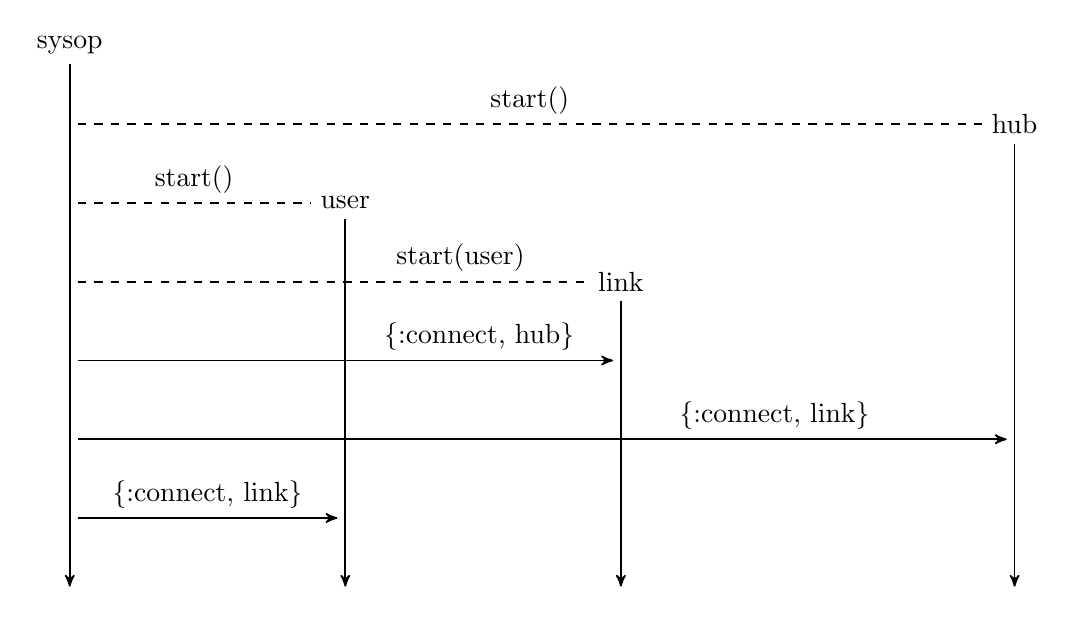
\begin{tikzpicture}[>=stealth', semithick, auto]

    \node[] (sysop) at (1,8) {sysop};
    \node[] (sysopn) at (1,1) {};
    \draw[->] (sysop) -- (sysopn);
    \pause
    \node[] (hub) at (13,7) {hub};
    \node[] (hubn) at (13,1) {};
    \draw[->] (hub) -- (hubn);

    \draw[dashed] (1.1,7) -- node[above] {start()} (hub);
    \pause
    
    \node[] (user) at (4.5,6) {user};
    \node[] (usern) at (4.5,1) {};    
    \draw[->] (user) -- (usern);

    \draw[dashed] (1.1,6) -- node[above] {start()}  (user);
    \pause
    
    \node[] (link) at (8,5) {link};
    \node[] (linkn) at (8,1) {};    
    \draw[->] (link) -- (linkn);

    \draw[dashed] (1.1,5) -- node[above, near end] {start(user)} (link);
    \pause
    
    \draw[->] (1.1,4) -- node[above, near end] {\{:connect, hub\}} (7.9,4);
    \pause
    \draw[->] (1.1,3) -- node[above, near end] {\{:connect, link\}} (12.9,3);
    \pause
    \draw[->] (1.1,2) -- node[above] {\{:connect, link\}} (4.4,2);    
    
    
  \end{tikzpicture}
  
  
\end{frame}

\begin{frame}{the network layer}


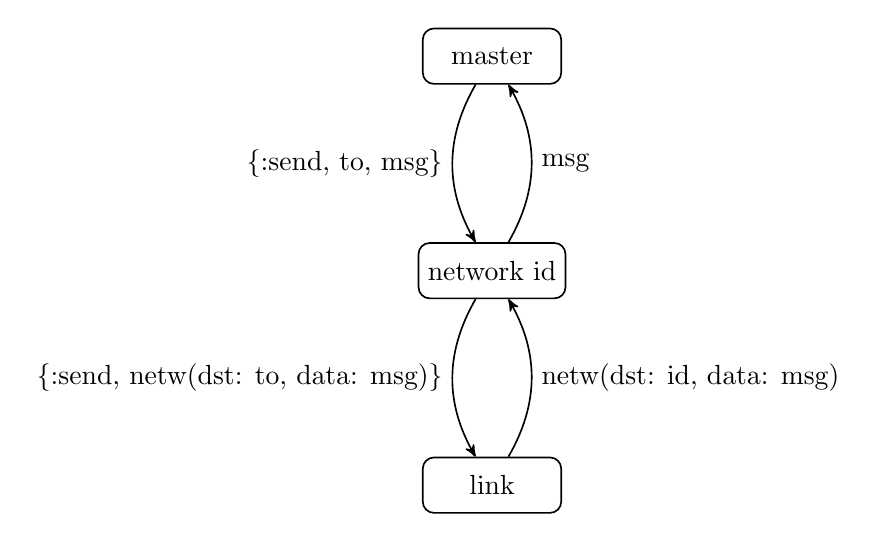
\begin{tikzpicture}[>=stealth', semithick, auto]

    \tikzstyle{fbp} = [rectangle, rounded corners, minimum width=50pt, minimum height=20pt, text centered, draw=black]        


    \node (master)  [fbp]                                 {master};

    \node (network)  [fbp, below=2cm of master]            {network id};

    \node (link)  [fbp, below=2cm of network]            {link};    


    \path[->, bend right]  (master)  edge  node[anchor=east]          {\{:send, to,  msg\}}                      (network);
    \path[->, bend right]  (network) edge  node[anchor=west]          {msg}                                      (master);
    \path[->, bend right]  (network) edge  node[anchor=east]          {\{:send, netw(dst: to,  data: msg)\}} (link);
    \path[->, bend right]  (link)    edge  node[anchor=west]          {netw(dst: id,  data: msg)}          (network);    
\end{tikzpicture}


\pause
\vspace{20pt}{\em The network layer will only forward messages with the right destination.}

\end{frame}


\begin{frame}{network process - a state diagram}
  
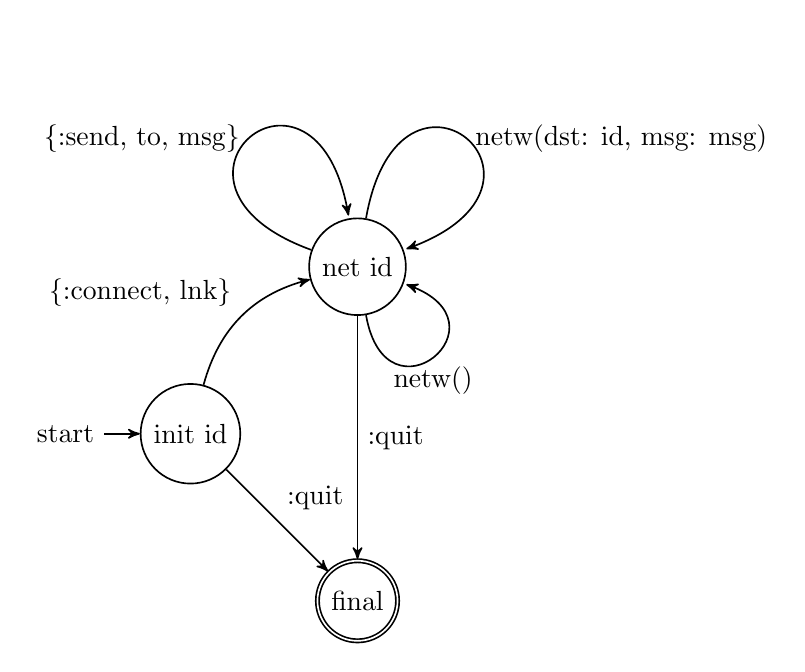
\begin{tikzpicture}[>=stealth', node distance=3cm, semithick, auto]

    \node[initial, state]   (init)                             {init id};
    \node[state]            (net)    [above right of=init]     {net id};
    \node[accepting, state] (final)  [below right of=init]     {final};

    
    \path[->]   (init)   edge       [bend left]     node      {\{:connect, lnk\}}       (net)
                         edge       []             node       {:quit}                   (final)
                (net)    edge       [loop above, every loop/.append style={looseness=10,in=20, out=80 }]   node[anchor=west] {netw(dst: id, msg: msg)}(net)
                         edge       [loop above, every loop/.append style={looseness=10,in=100, out=160 }] node[anchor=east] {\{:send, to, msg\}}    (net)
                         edge       [loop below, every loop/.append style={looseness=6,in=340, out=280 }]  node              {netw()}             (net)
                         edge       []                                                                     node              {:quit}                 (final);
    
\end{tikzpicture}
\end{frame}

\begin{frame}[fragile]{the network process}

\begin{verbatim}
def network(master, id, link) do
   receive do
     {:send, to, msg} ->
       send(link, {:send, netw(src: id, dst: to,  data: msg)})
       network(master, id, link)

     netw(dst: ^id, data: msg) ->
       send(master, msg)
       network(master, id, link)

     netw() ->
       network(master, id, link)

     :quit ->
       :ok
   end
 end
\end{verbatim}
  
\end{frame}


\begin{frame}{order and reliability}

\pause A {\em communication channel} is a duplex flow of an ordered sequence of messages. 

\pause 
 \vspace{20pt}
 \begin{itemize}
  \item add a sequence number to each message \pause
  \item order messages as they arrive and \pause
  \item resend lost messages
\end{itemize}

\end{frame}

\begin{frame}{the order layer}

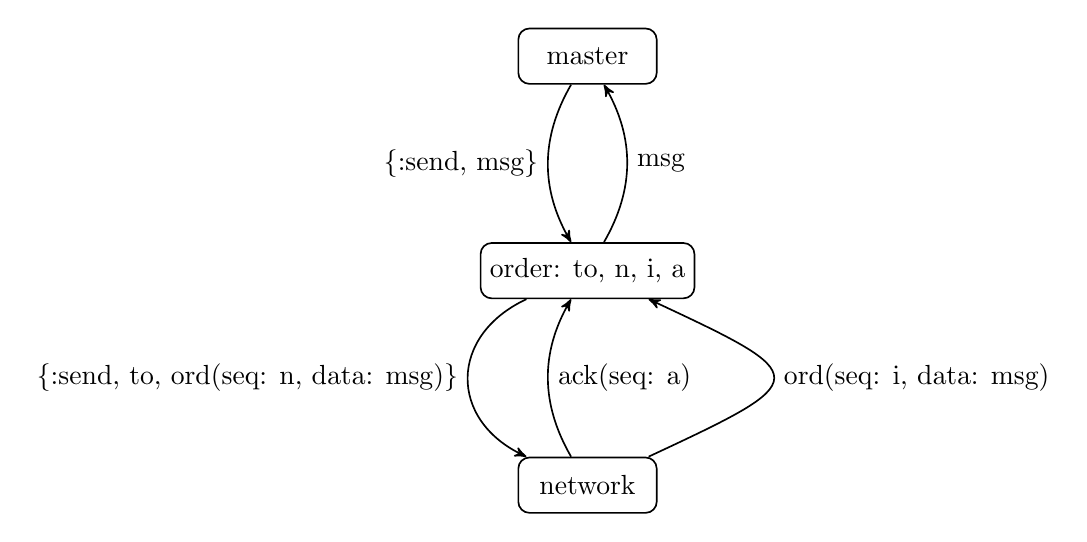
\begin{tikzpicture}[>=stealth', semithick, auto]

    \tikzstyle{fbp} = [rectangle, rounded corners, minimum width=50pt, minimum height=20pt, text centered, draw=black]        


    \node (master)   [fbp]                        {master};

    \node (order)    [fbp, below=2cm of master]   {order: to, n, i, a};

    \node (network)  [fbp, below=2cm of order]    {network};    


    \path[->, bend right]  (master)   edge     node[anchor=east]    {\{:send, msg\}}                            (order);
    \path[->, bend right]  (order)    edge     node[anchor=west]    {msg}                                       (master);

    \path[->, bend right=65, looseness=1.4]  (order)    edge     node[anchor=east]    {\{:send, to, ord(seq: n, data: msg)\}} (network);
    \path[->, bend right=65, looseness=3]  (network)  edge     node[anchor=west]    {ord(seq: i,  data: msg)}               (order);    
    \path[->, bend left]              (network)  edge     node[anchor=west]    {ack(seq: a)}                          (order);    
\end{tikzpicture}

\pause
\vspace{20pt}{\em The layer will need to buffer messages and use a timeout to detect missing datagrams.}

\end{frame}


\begin{frame}{the sending process - state diagram}
  
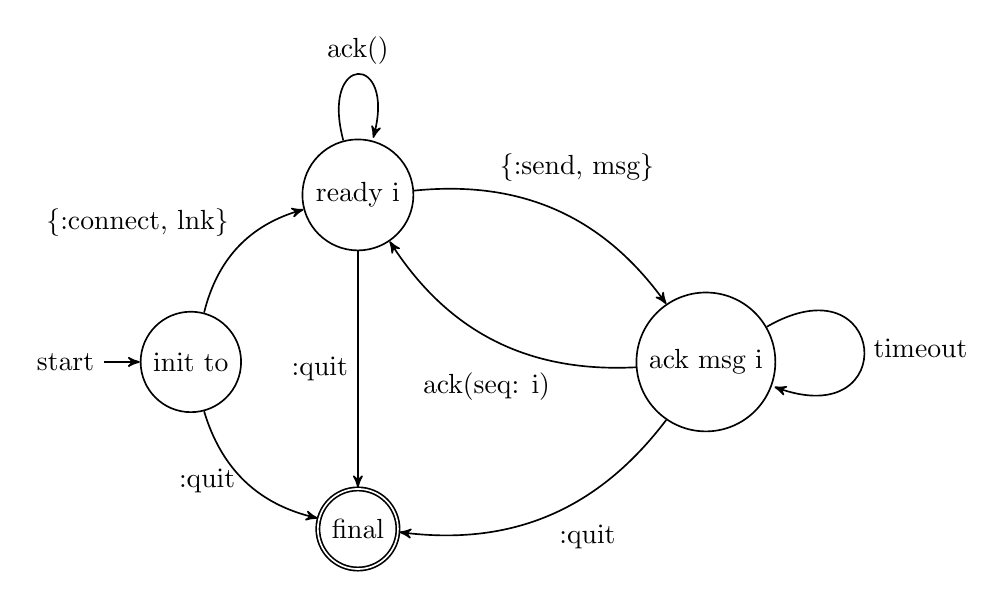
\begin{tikzpicture}[scale=1, >=stealth', node distance=3cm, semithick, auto]
    \node[initial, state]            (init)                              {init to};
    \node[state]                     (ready)   [above right of=init]     {ready i};
    \node[state]                     (send)    [right=5cm of init]    {ack msg i};
    \node[accepting, state]          (final)   [below right of=init]     {final};

    
    \path[->]   (init)   edge       [bend left]  node                                  {\{:connect, lnk\}}   (ready)
                         edge       [bend right] node[anchor=east]                     {:quit}               (final)
                (ready)  edge       [bend left]  node[anchor=south west, near start]   {\{:send, msg\}}      (send)
                         edge       [loop above] node                                  {ack()}           (ready)
                         edge       [] node[anchor=east]                               {:quit}               (final)              
                (send)   edge       [loop below, every loop/.append style={looseness=6,in=340, out=30 }] node[anchor=west] {timeout}  (send)   
                         edge       [bend left]  node[near start, anchor=north east]   {ack(seq: i)}     (ready)
                         edge       [bend left]  node                                  {:quit}               (final);
\end{tikzpicture}
  
\end{frame}


\begin{frame}{the receiving process - state diagram}

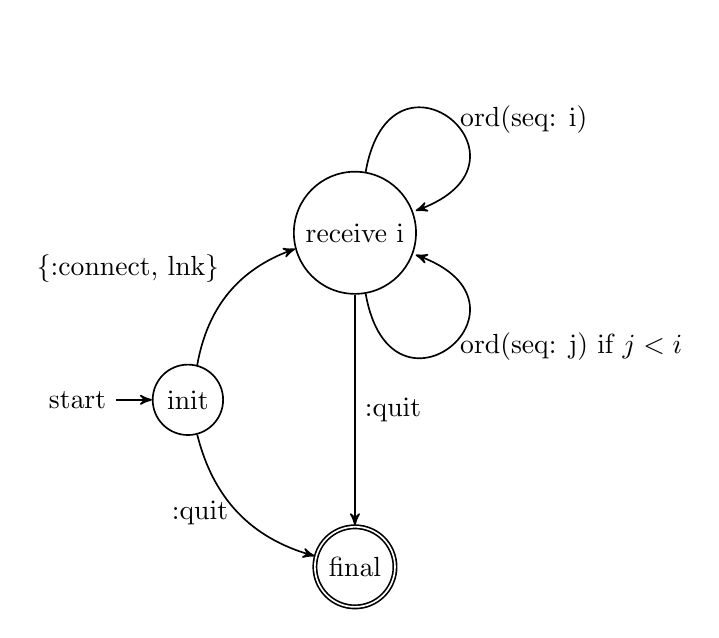
\begin{tikzpicture}[scale=1,>=stealth', node distance=3cm, semithick, auto]
    \node[initial, state]            (init)                              {init};
    \node[state]                     (receive) [above right of=init]     {receive i};
    \node[accepting, state]          (final)   [below right of=init]     {final};

    
    \path[->]   (init)   edge       [bend left]                  node              {\{:connect, lnk\}}   (receive)
                         edge       [below, bend right]          node[anchor=east] {:quit}               (final)
               (receive)   edge     [loop above, every loop/.append style={looseness=6,in=20, out=80}]   node[anchor=west] {ord(seq: i)} (receive)
                         edge       [loop below, every loop/.append style={looseness=6,in=340, out=280}] node[anchor=west] {ord(seq: j) if $j<i$}  (receive)
                         edge       []                                                                   node              {:quit}                   (final);
\end{tikzpicture}
  
\end{frame}


\begin{frame}[fragile]{the order process}

\begin{verbatim}
  def order(master, to, n, i, [], netw) do
    receive do
      ord(seq: ^i, data: msg) ->
        send(netw, {:send, to, ack(seq: i)})
        send(master, msg)
        order(master, to, n, i+1, [], netw)
        
      :
         
      {:send, msg} ->
        send(netw, {:send, to, ord(seq: n, data: msg)})
        order(master, to, n+1, i, [{n, msg}], netw);
    end
  end
\end{verbatim}
  
\end{frame}

\begin{frame}[fragile]{the order process}

\begin{verbatim}
  def order(master, to, n, i, [{a,res}|rest]=buffer, netw) do
    receive do
       :
      ack(seq: ^a) ->
        order(master, to, n, i, rest, netw)

       :

       :
                
    after 10 ->
        dgr = ord(seq: a, data: res)
        send(netw, {:send, to, dgr})
        order(master, to, n, i, buffer, netw)
    end
\end{verbatim}
\end{frame}

\begin{frame}{flow control}

 \begin{itemize}
  \item do not overflow the receiver \pause
  \item keep track of the reciever buffer size  \pause
  \item wait for the user to activly read messges \pause
\end{itemize}

\vspace{20pt}{\em We are introducing a synchronous interface - only send if receiver prepared.}

\end{frame}

\begin{frame}{the flow control}

  \begin{itemize}
  \item {\tt \{:send, msg, pid\}} 

  \item {\tt \{:read, n, pid\}} 


  \item {\tt msg(data: msg)}

  \item {\tt syn(add: a)}

      
\end{itemize}
  
\end{frame}

\begin{frame}{the flow control }

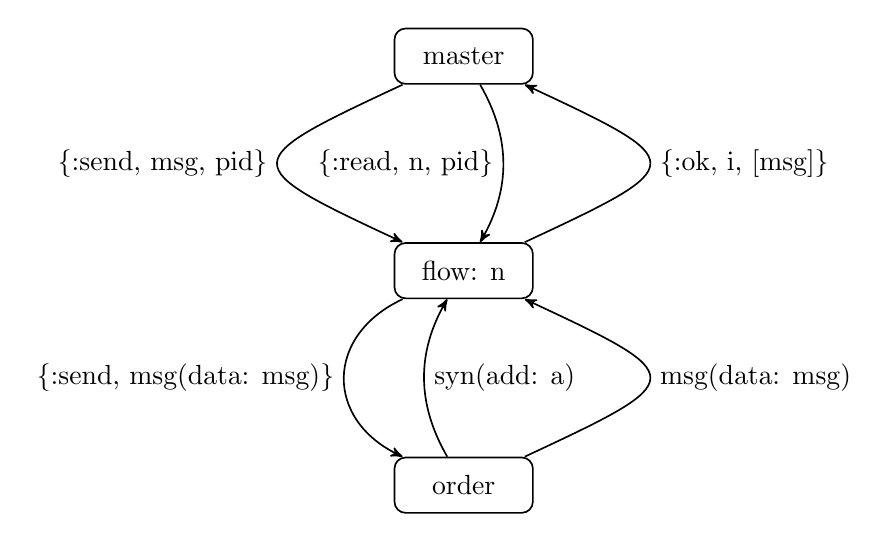
\begin{tikzpicture}[>=stealth', semithick, auto]

    \tikzstyle{fbp} = [rectangle, rounded corners, minimum width=50pt, minimum height=20pt, text centered, draw=black]        


    \node (master)   [fbp]                        {master};

    \node (flow)    [fbp, below=2cm of master]   {flow: n};

    \node (order)  [fbp, below=2cm of flow]    {order};    


    \path[->, bend right=65, looseness=3]  (master)  edge     node[anchor=east]    {\{:send, msg, pid\}}                            (flow);
    \path[->, bend left]  (master)  edge     node[anchor=east]    {\{:read, n, pid\}}                         (flow);    
    \path[->, bend right=65, looseness=3]  (flow)    edge     node[anchor=west]    {\{:ok, i, [msg]\}}                          (master);

    \path[->, bend right=65, looseness=1.4]  (flow)    edge     node[anchor=east]    {\{:send, msg(data: msg)\}} (order);
    \path[->, bend right=65, looseness=3]  (order)  edge     node[anchor=west]    {msg(data: msg)}               (flow);    
    \path[->, bend left]              (order)  edge     node[anchor=west]    {syn(add: a)}                          (flow);    
\end{tikzpicture}
  
  
\end{frame}

\begin{frame}{the flow sending process}

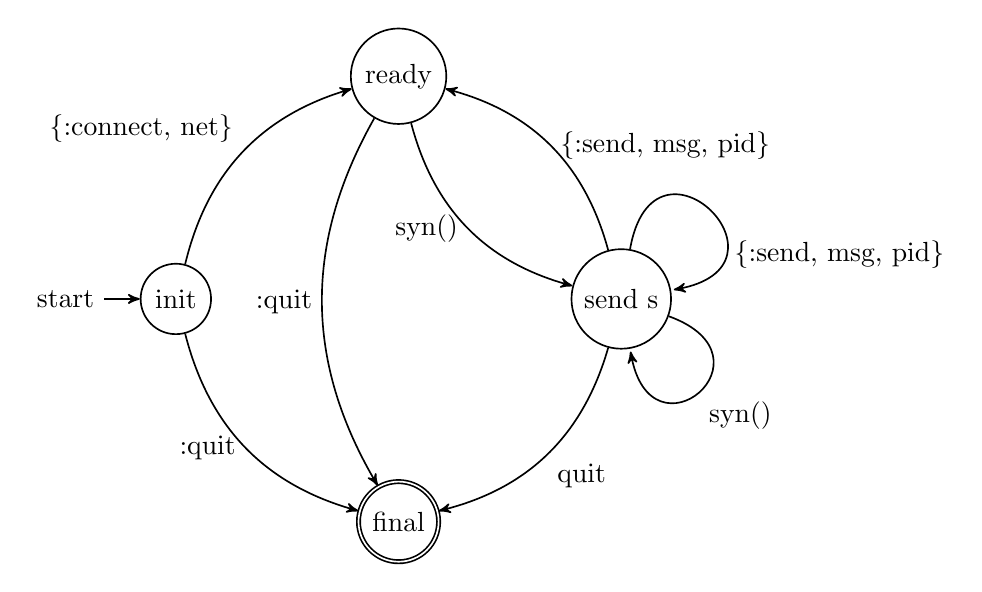
\begin{tikzpicture}[scale=1, >=stealth', node distance=4cm, semithick, auto]
    \node[initial, state]            (init)                              {init};
    \node[state]                     (ready)   [above right of=init]     {ready};
    \node[state]                     (send)   [below right of=ready]     {send s};
    \node[accepting, state]          (final)   [below right of=init]     {final};

    
    \path[->]   (init)   edge       [bend left]  node               {\{:connect, net\}}       (ready)
                         edge       [bend right] node[anchor=east]  {:quit}                   (final)
                (ready)  edge       [bend right] node[anchor=east]  {syn()}               (send)
                         edge       [bend right] node[anchor=east]  {:quit}                   (final)                   
                (send)   edge       [bend right] node[anchor=west]  {\{:send, msg, pid\}}      (ready)
                         edge       [loop below, every loop/.append style={looseness=6,out=80, in=10 }]   node[anchor=west, near end]  {{\{:send, msg, pid\}}}   (send)   
                         edge       [loop below, every loop/.append style={looseness=6,out=340, in=280 }] node[anchor=north west] {syn()}     (send)
                         edge       [bend left]               node  {quit}    (final);
\end{tikzpicture}
  
  
\end{frame}


\begin{frame}{the flow receiving process}
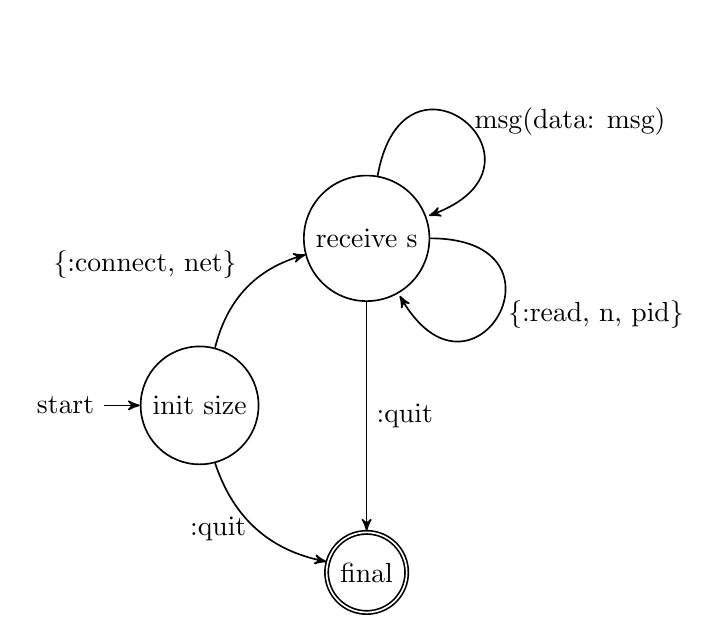
\begin{tikzpicture}[scale=1,>=stealth', node distance=3cm, semithick, auto]
    \node[initial, state]            (init)                              {init size};
    \node[state]                     (receive)   [above right of=init]   {receive s};
    \node[accepting, state]          (final)   [below right of=init]     {final};

    
    \path[->]   (init)   edge  [bend left]     node                  {\{:connect, net\}}        (receive)
                         edge  [below, bend right] node[anchor=east] {:quit}                    (final)
              (receive)  edge  [loop above, every loop/.append style={looseness=6,in=20, out=80 }] node[anchor=west]   {msg(data: msg)}   (receive)
                         edge  [loop above, every loop/.append style={looseness=6,in=300, out=0 }] node[anchor=west]   {\{:read, n, pid\}}     (receive)
                         edge  []              node                  {:quit}                    (final);
\end{tikzpicture}
\end{frame}

\begin{frame}{extensions}

\begin{itemize}
  \item What if the link layer could only send sequences of bytes?  \pause
  \item Can we add error detection in the link layer? \pause
  \item Could we build a switch or router? \pause
\end{itemize}

\end{frame}

\begin{frame}{a switch}

\includegraphics[scale=0.4]{switch.jpg}

\end{frame}


\begin{frame}{summary}

\pause
\begin{itemize}
 \item divide a service into processes \pause
 \item layers of abstraction \pause
 \item finite State Machine (FSM) description of a process \pause
 \item sequence diagrams to show protocol \pause
 \item asynchronous and synchronous interfaces \pause
\end{itemize}

\vspace{20pt}{\em .. and hopefully, you have learned about communication stacks}
\end{frame}

\end{document}



